\documentclass[a4paper,12pt]{article}
\usepackage[slovene]{babel}
\usepackage[utf8]{inputenc}
\usepackage[T1]{fontenc}
\usepackage{lmodern}

\usepackage{float}
\usepackage{url}
\usepackage[]{amsmath}
\usepackage[]{amsthm}
\usepackage[]{graphicx}
\usepackage{amssymb}

\newcommand{\pojem}[1]{\underline{\textsc{#1}}}

\theoremstyle{definition}
\newtheorem{definicija}{Definicija}

\theoremstyle{plain}
\newtheorem{izrek}{Izrek}

\newenvironment{dokaz}{\begin{proof}[Dokaz izreka]}{\end{proof}}




\begin{document}

\begin{titlepage}

\title{The triangle scheduling problem}
\author{Arh Blaž, Matušek Matic}
\date{9.\ 11.\ 2022}
\maketitle   
\thispagestyle{empty}
\end{titlepage}

\section{Uvod}
\subsection{Problem}

Imamo $n$ pravokotnih enakokrakih trikotnikov, ki so določeni z dolžino kraka $d_i$ za $i=1,2,...,n$  in pravim kotom med krakoma. Postavljamo jih z nogo na $x$-os na sledeči način:
\begin{center}
   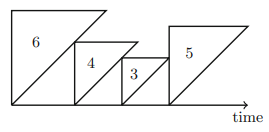
\includegraphics[width=8cm, height=4cm]{primer_trikotnikov.png} 
\end{center}
Želimo si trikotnike postaviti tako, da je dolžina teh trikotnikov najkrajša. Trikotniki se med seboj ne smejo prekrivati,
prav tako pa mora biti krak noge pravokoten na $x$-os

\subsection{Uporabnost}
Želimo si sestaviti urnik iz $n$ opravil. Naj bo $d_i$ pomembnost $i$-tega opravila. Radi bi dosegli čim krajši urnik. Želimo, da se pomembnejša opravila izvedejo, v primeru zakasnitve le teh pa lahko manj pomembna opravila izpustimo.
Večji kot je trikotnik, bolj pomembno je opravilo. Kot je razvidno iz zgornje slike, lahko opravila z manjšo pomembnostjo vstavimo pod opravila z večjo pomembnostjo. To pomeni, da manjše trikotnike vstavljamo pod večje. Torej, če pride do zakasnitve
pomembnejšega opravila (večjega trikotnika), manj pomembno opravilo  izpustimo (manjši trikotnik).

\newpage
\section{Greedy algoritem}
Greedy algoritem je kateri koli algoritem, ki rešuje problem tako, da na vsakem koraku naredi lokalno optimalno izbiro. Pri številnih problemih Greedy algoritem ne ustvari optimalne rešitve, prav tako ne pri našem problemu. 
Greedy algoritem najprej razvrsti trikotnike tako, da velja \newline
$d_1 \geq d_2 \geq d_3 \geq ... \geq d_n$. Prvi trikotnik razvrsti na $x=0$, kar ustvari prostor pod trikotnikom 1.
Nato vsak trikotnik $j=2,...,n$ postavi v največji možen prostor pod že postavljenimi trikotniki. Če je več enakih prostorov, izbere prvega povrsti.
Če ima izbrani prostor pod trikotnikom dolžino $l$ in se začne v času $x_i$, potem je trikotnik $j$ postavljen na mesto $x_j=x_i+d_j$. Če je $2d_j \ge l$  potem se vsi trikotniki $k$, za katere je $x_k \ge x_j$ zamaknejo za $ 2d_j-l$, da se ne prekrivajo. Opisano 
dogajanje prikazuje spodnji primer:
\begin{center}
    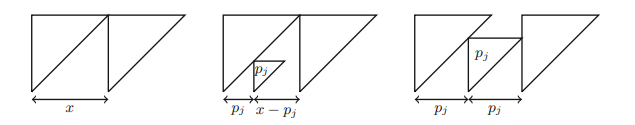
\includegraphics[width=13cm, height=3cm]{greedy.png} 
 \end{center}
Na naslednji sliki prikažemo primer ko Greedy ni optimalen. Greedy algoritem (desna slika) vrne dolzino 42 in ne vrne optimalne dolžine, ki je 40 (leva slika):
\begin{center}
    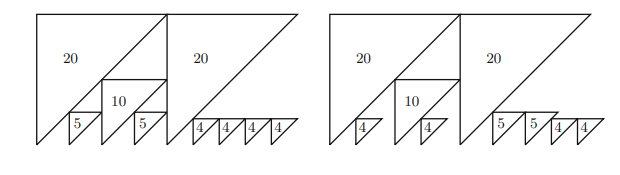
\includegraphics[width=10cm, height=3cm]{primer_neoptimalnosti_greedy.png} 
 \end{center}
Hitrost Greedy algoritma je polinomska. Da se pokazati, da je aproksimacijsko razmerje zgornje meje točnosti Greedy algoritma $1.5$ optimalnega časa. Torej, če je optimalni čas določenega primerna
$40$ časovnih enot, potem Greedy pokaže največ $60$ časovnih enot.

\section{Načrt dela}
Za zdaj sva naredila program, ki ustvari trikotnike in jih razporedi na \newline $x$-os. Prav tako sva naredila brute force algoritem, da lahko svoje rezultate preveriva.
V nadaljevanju bova napisala še Greedy algoritem in še algoritem, ki poišče optimalno rešitev hitreje kot brute force algoritem.


\end{document}







